\documentclass[journal]{IEEEtran}
\usepackage{amsmath,amssymb,amsthm}
\usepackage{graphicx}
\usepackage{booktabs}
\usepackage{multirow}
\usepackage{array}
\usepackage{algorithm}
\usepackage{algorithmic}
\usepackage{xcolor}
\usepackage{cite}
\usepackage{url}
\usepackage{textcomp}
\makeatletter
\setlength{\@fptop}{0pt}
\makeatother
\begin{document}
\title{Supplementary Information for ``PC-AVCT: Context-Augmented, Session-Calibrated Blood Pressure Tracking from PPG''}
\author{Farouk~Ganiyu~Adewumi~and~Timothy~Oladunni}
\maketitle
\noindent This document contains implementation details, historical development analyses, negative results, clinical-standards context, and regenerated subgroup diagnostics supporting the main manuscript. Primary claims and conclusions are reported in the main manuscript.
\appendices
\section{Supplementary Implementation Details}
\label{app:implementation}
\setcounter{table}{0}\renewcommand{\thetable}{S\arabic{table}}
\setcounter{figure}{0}\renewcommand{\thefigure}{S\arabic{figure}}
\subsection{Multi-Wavelength Pulse Processing}
For each device, visible and infrared pulse rates are estimated around the scheduled reference time using a window of up to 12~s, with at least 7.5~s and 150 samples required. Timestamps are converted to seconds, sorted, and deduplicated; signals are interpolated to a uniform grid using the median interval, with inferred sampling rate clipped to 20--500~Hz. A third-order 0.55--4~Hz Butterworth filter is applied forward and backward after detrending. Welch spectra use up to 8~s segments (at least 256 samples when available), with 50\% overlap. The dominant frequency is sought in 0.65--3.5~Hz; spectral concentration $c$ is the fraction of pulse-band power within 0.18~Hz of that peak.

An autocorrelation pulse estimate searches lags corresponding to 39--210~BPM. Let $a$ be the selected autocorrelation peak clipped to $[0,1]$, and $h_F,h_A$ the spectral and autocorrelation rates. When $|h_F-h_A|\leq15$~BPM, the channel estimate is $(c h_F+a h_A)/(c+a)$; otherwise the estimate with the larger reliability component is used. Channel quality is
\begin{align}
q&=\operatorname{clip}\!\left(\sqrt{ca}\,g,10^{-4},1\right),\\
g&=\begin{cases}1,&|h_F-h_A|\leq15,\\
e^{-|h_F-h_A|/30},&\text{otherwise.}\end{cases}
\end{align}
The tone-blind fusion estimate is $(q_Vh_V+q_Ih_I)/(q_V+q_I)$. The optional tone-dependent arm replaces the weights by $q_Ve^{-\alpha z}$ and $q_Ie^{\alpha z}$, with $z=\operatorname{clip}[(\mathrm{MST}-1)/9,0,1]$. Candidate $\alpha$ values are $\{0,\pm0.25,\pm0.5,\pm0.75,\pm1,\pm1.5,\pm2,\pm3\}$. Four participant folds within each outer training set score these fixed candidate rules. The selected nonzero exponent must improve mean fold MAE by at least 0.10~BPM and improve every inner fold; otherwise $\alpha=0$. The seed is 20260827, with repeat/fold offsets defined in the companion script. These methods estimate pulse rate, not BP.

\subsection{VitalDB Extraction and Model Selection}
Eligible cases have all three required tracks and a case duration of at least 1,800~s. Cases are deterministically shuffled with seed 20260827; positions 1--60 define development and 61--300 define the candidate holdout. The saved audit contains 55 development cases/subjects and 228 eligible holdout cases from 227 subjects, with no subject overlap. Eligibility and sampling are retrospective, and selecting windows across the completed record is not an online scheduling policy.

Candidate centers start no earlier than 120~s, proceed in 30-s increments, and require at least 900~s of usable overlapping record. PPG is retained at approximately 100~Hz. A 20-s window must contain at least 75\% of the expected samples and 85\% finite values; gaps are interpolated. Values are clipped to the median plus/minus eight robust SD estimates, detrended, and filtered with a third-order 0.5--8~Hz bandpass (upper cutoff limited by sampling rate). Pulse quality is spectral concentration multiplied by $\exp[-\min(\mathrm{interval\ CV},2)]$; windows below 0.04 are excluded. Pulse frequency search, spectral concentration, and beat-interval limits follow the companion extraction code. This quality filter is held fixed, but a no-quality-filter ablation is not reported.

Reference BP is the median of at least three plausible values within $\pm5$~s of the center. SBP must lie in 70--220~mmHg and DBP in 35--130~mmHg; local robust SD must not exceed 8 and 6~mmHg, respectively. Pulse pressure must lie in 20--130~mmHg. These reference-based exclusions do not use prediction errors but restrict the evaluated BP distribution. Cases require at least eight valid windows. The first three define median BP and feature anchors; up to 24 later windows are selected using evenly spaced indices over the valid future windows.

The context model uses anchor BP, $\log(1+\mathrm{elapsed\ seconds})$, age, sex, and preoperative hypertension (missing hypertension is coded as zero). The PPG model adds current and calibration-relative optical features listed by the \texttt{columns} function in the companion script. Candidate estimators comprise standardized ridge regression with 13 logarithmically spaced penalties from $10^{-3}$ to $10^3$ and three absolute-loss gradient-boosting configurations. Development-only five-fold participant validation selects estimators, followed by a fixed blend weight from $\{0,0.25,0.5,0.75,1\}$; a nonzero weight requires at least 0.10~mmHg improvement over context. Development selection is not independently nested across the estimator and blend choices, but holdout observations are excluded from both. Delta predictions are clipped at training-target 1st/99th percentiles.

Both endpoints selected ridge context models with penalty approximately 31.6228. The SBP PPG model uses absolute-loss boosting, learning rate 0.03, 15 leaves, regularization 5, 250 iterations, and minimum leaf size 20; the DBP PPG model uses ridge with penalty approximately 31.6228. Both selected a constant 0.5 PPG weight. The saved predictions satisfy this fixed-blend identity to numerical precision. Errors are averaged over all windows from all cases of a subject before subject bootstrap; the subject contributing two cases remains one bootstrap unit.

\subsection{Audit Scope and Reproduction Status}
The independent-dataset saved-result audit uses 10,000 participant bootstrap resamples with seed 20260910 for the pulse comparisons and verifies window uniqueness, case/subject counts, development/holdout separation, the fixed VitalDB blend, and the pulse-fusion equation. The AuroraBP analysis was separately rerun: the context arms and all three calibration doses were refitted across three repeats of five participant folds. The package records hashed feature inputs, software versions, selected features and gates, row-level outer-fold predictions, and paired participant contrasts. The historical subgroup model was also refitted. The rerun starts from feature banks; raw-waveform extraction is outside its scope.

\begin{table*}[t]
\centering
\caption{Interventions Tested and Not Adopted (Elimination Log)}
\label{tab:whatdidnotwork}
\begin{tabular}{p{4.6cm}p{2.4cm}p{7.8cm}}
\toprule
Intervention & Times tested & Outcome \\
\midrule
Absolute-error loss (vs.\ squared) & 3 & Never CI-supported: $+0.152$ [$-0.001$, 0.311] (51.8\% helped); $+0.102$ [$-0.028$, 0.240]; $+0.163$ [$-0.008$, 0.345] (exactly 50.0\% helped). \\
HCA feature augmentation & 2 & No CI-supported benefit: $-0.077$ [$-0.183$, 0.024]; $+0.043$ [$-0.026$, 0.115] (53.0\% helped). \\
Signal-level pigmentation (Beer--Lambert) correction & 2 & First variant increased error; the repeated-CV corrected channel changed MAE by $-0.007$ [$-0.042$, 0.029] SBP and $-0.030$ [$-0.062$, 0.003] DBP -- no established overall benefit (the main manuscript's repeated-CV pigmentation-correction subsection). \\
Demographic (Fitzpatrick-band) rebalancing / group gating & 5 & Consistently harmful: e.g., $-0.291$ [$-0.420,-0.170]$ mmHg SBP; widens between-band gap in every run (the main manuscript's Secondary Pigmentation-Intervention Audit). \\
Multi-window feature averaging & 1 & No measurable benefit; nominally worse (Section~\ref{sec:multiwindow}). \\
Nested gate/threshold search (early pipeline) & 1 & Higher error than a plainer reference baseline (8.253/8.183 vs.\ 8.109~mmHg SBP). \\
\midrule
\emph{Passed sanity check:} metadata-only permutation control & 1 & AUC $=0.492$ ($\approx$ chance) -- is consistent with chance under this permutation control; does not exclude other confounds. \\
\bottomrule
\end{tabular}
\end{table*}
\section{Historical Development and Auxiliary Analyses}
The following analyses preserve the development record. They are secondary or exploratory. The final subgroup subsection reports newly refitted estimates; development codes C0--C4 refer to the historical arms.
\subsection{Exploratory Endpoint-Specific Calibration and Warning Router}
\label{sec:v34}
Table~\ref{tab:v33primary} reports the historical post-primary endpoint analysis retained from the development record; it was not refitted in the V38 primary rerun. A nested, tightly clipped residual calibrator reduced SBP participant-level MAE from $7.611$ to $7.555$~mmHg, a paired improvement of $0.056$~mmHg (95\% CI $0.020$--$0.091$; $55.9\%$ of participants helped). The absolute gain is small, and tail behavior changed little (P90 absolute error $16.862 \to 16.820$~mmHg; P95 $22.184 \to 22.120$~mmHg). DBP candidate specialization did not improve inner-fold performance consistently, so the base prediction was retained at $5.784$~mmHg. This endpoint-specific policy is more conservative than adopting one post-processing rule for both targets.
\begin{table}[t]
\centering
\caption{Exploratory Endpoint-Specific Nested Analysis (653 Participants)}
\label{tab:v33primary}
\scriptsize
\resizebox{\columnwidth}{!}{%
\begin{tabular}{llrrr}
\toprule
Target & Arm & MAE & P90 AE & P95 AE \\
\midrule
SBP & Base & 7.611 & 16.862 & 22.184 \\
SBP & Clipped residual & \textbf{7.555} & 16.820 & 22.120 \\
DBP & Base & 5.784 & 12.043 & 15.630 \\
DBP & Selected policy & 5.784 & 12.043 & 15.630 \\
\midrule
\multicolumn{5}{l}{\footnotesize SBP paired gain: 0.056 mmHg [0.020, 0.091]; DBP gain: 0.000.} \\
\bottomrule
\end{tabular}
}
\end{table}
The exploratory DBP router was therefore frozen as warning-only. Extreme DBP change prevalence was $20.5\%$ (95\% CI $19.1$--$21.9\%$). The router achieved ROC AUC $0.794$ ($0.778$--$0.809$), average precision $0.517$ ($0.483$--$0.555$), and Brier score $0.130$ ($0.122$--$0.137$). At the nested operating threshold, warning precision was $0.773$ ($0.695$--$0.854$), but recall was only $0.043$ ($0.035$--$0.052$) and the warning rate was $1.1\%$ ($0.9$--$1.4\%$). The router is thus a rare high-precision flag at the evaluated threshold; it is not a screen for most extreme changes, does not reduce reported DBP MAE, and must not be interpreted as a clinical safety mechanism.
\subsection{Historical Duplicate-Reading Noise Diagnostic}
Table~\ref{tab:noisefloor} retains a historical duplicate-reading diagnostic, not a universal achievable-error bound. Estimating per-reading noise as $\sigma_{P-S}/\sqrt{2}$ assumes independent, equal-variance observer errors. The supplied code distinguishes a stored average of two readings from a single-reading target and propagates target and anchor errors for a legacy two-time-point difference. Its $1.754$/$2.412$~mmHg Gaussian absolute-noise estimates and $2.6\%$/$9.2\%$ variance ratios therefore must not be treated as validated floors for the primary three-reading anchor. Shared observer error, physiological change during measurement, and the actual target-averaging rule can change the estimates. A primary-endpoint noise calculation would require those components and their covariances; subtracting a putative floor from model MAE does not measure recoverable physiological error.
\begin{table}[t]
\centering
\caption{Historical Duplicate-Reading Diagnostic (8{,}918/8{,}916 SBP/DBP pairs)}
\label{tab:noisefloor}
\begin{tabular}{lrr}
\toprule
Quantity (mmHg) & SBP & DBP \\
\midrule
$\sigma$(primary $-$ secondary reading) & 3.108 & 4.275 \\
$\sigma_{\mathrm{cuff}}$ (per-reading noise) & 2.198 & 3.023 \\
Legacy Gaussian absolute-noise estimate & 1.754 & 2.412 \\
Observed SD of $\Delta$ & 13.70 & 9.98 \\
Legacy noise/observed variance ratio & 2.6\% & 9.2\% \\
Residual SD under legacy assumptions & 13.52 & 9.51 \\
Early reference model MAE & 8.11 & -- \\
\bottomrule
\end{tabular}
\end{table}
\subsection{Recalibration Cadence}
The historical code evaluated nominal recalibration intervals of 1, 3, 6, 12, and 24~h, with nearly identical MAE ($8.593$--$8.594$~mmHg SBP; $6.020$--$6.022$~mmHg DBP). Those labels do not establish distinct effective recalibration schedules in the analyzed short laboratory sessions. The stored comparison lacks an event-count and elapsed-time audit sufficient to interpret a cadence effect. We therefore withdraw the inference that cadence beyond one hour is immaterial and make no recommendation about recalibration frequency from this analysis.
\subsection{Multi-Window Feature Averaging}
\label{sec:multiwindow}
Averaging attractor features over multiple 10~s windows per recording (up to 3 available) was hypothesized to reduce measurement noise (Table~\ref{tab:multiwindow} shows within/between SD ratios up to approximately 0.45). It did not help: holdout MAE with multi-window averaging ($6.393$/$4.828$~mmHg SBP/DBP) was statistically indistinguishable from, and nominally slightly worse than, a matched single-window configuration ($6.346$/$4.803$~mmHg), both close to the legacy single-window baseline ($6.315$/$4.789$~mmHg). We report this as a negative result (Table~\ref{tab:whatdidnotwork}).
\begin{table}[t]
\centering
\caption{Historical Within- and Between-Recording Feature SD}
\label{tab:multiwindow}
\begin{tabular}{lrrr}
\toprule
Feature & Within SD & Between SD & SD ratio \\
\midrule
$\sigma_m$ & 0.0046 & 0.0102 & 0.449 \\
CSI & 0.0043 & 0.0138 & 0.311 \\
Recurrence rate & 0.0040 & 0.0130 & 0.305 \\
Kurtosis & 0.0902 & 0.3086 & 0.292 \\
RQA entropy & 0.0734 & 0.2520 & 0.291 \\
Skewness & 0.0386 & 0.1389 & 0.278 \\
Sample entropy & 0.0133 & 0.0527 & 0.252 \\
Determinism & 0.0114 & 0.0475 & 0.240 \\
Spectral entropy & 0.0092 & 0.0488 & 0.189 \\
Permutation entropy & 0.0028 & 0.0190 & 0.150 \\
\bottomrule
\end{tabular}
\end{table}

\subsection{Historical Fixed-Split Session-Anchored Ladder}
\label{sec:v23}
During earlier development, the model-development ladder was evaluated on a fixed 501/168 participant split. Table~\ref{tab:v23} preserves that analysis for transparency: C4 reduced MAE from $8.856$/$6.582$ to $7.147$/$5.579$~mmHg. Because the same 168 participants were examined across successive ablations, these values are historical development evidence and are not the paper's primary validation result. The corresponding repeated participant-validation estimates in the main manuscript's primary validation table are modestly worse ($7.523$/$5.743$~mmHg for protocol-enriched context), consistent with mild optimism from the fixed split rather than a collapse of the effect.
\begin{table}[t]
\centering
\caption{Historical Fixed-Split Session-Anchored Ladder (168 Evaluation Participants)}
\label{tab:v23}
\resizebox{\columnwidth}{!}{%
\begin{tabular}{lrrr}
\toprule
Arm & SBP MAE [95\% CI] & DBP MAE [95\% CI] \\
\midrule
Calibration retention & 8.856 & 6.582 \\
C0 legacy (squared) & 7.956 [7.424, 8.501] & 6.120 [5.641, 6.647] \\
C1 absolute loss & 7.793 [7.270, 8.316] & 6.014 [5.513, 6.546] \\
C2 +context & 7.156 [6.740, 7.618] & 5.651 [5.186, 6.146] \\
C3 +context+HCA & 7.113 [6.703, 7.550] & 5.636 [5.178, 6.126] \\
\textbf{C4 +context (squared)} & \textbf{7.147 [6.736, 7.593]} & \textbf{5.579 [5.174, 6.004]} \\
\midrule
Reduction, calib.\ $\rightarrow$ C4 & \textbf{1.709 (19.3\%)} & \textbf{1.003 (15.2\%)} \\
\bottomrule
\end{tabular}
}
\end{table}
\begin{figure}[t]
\centering
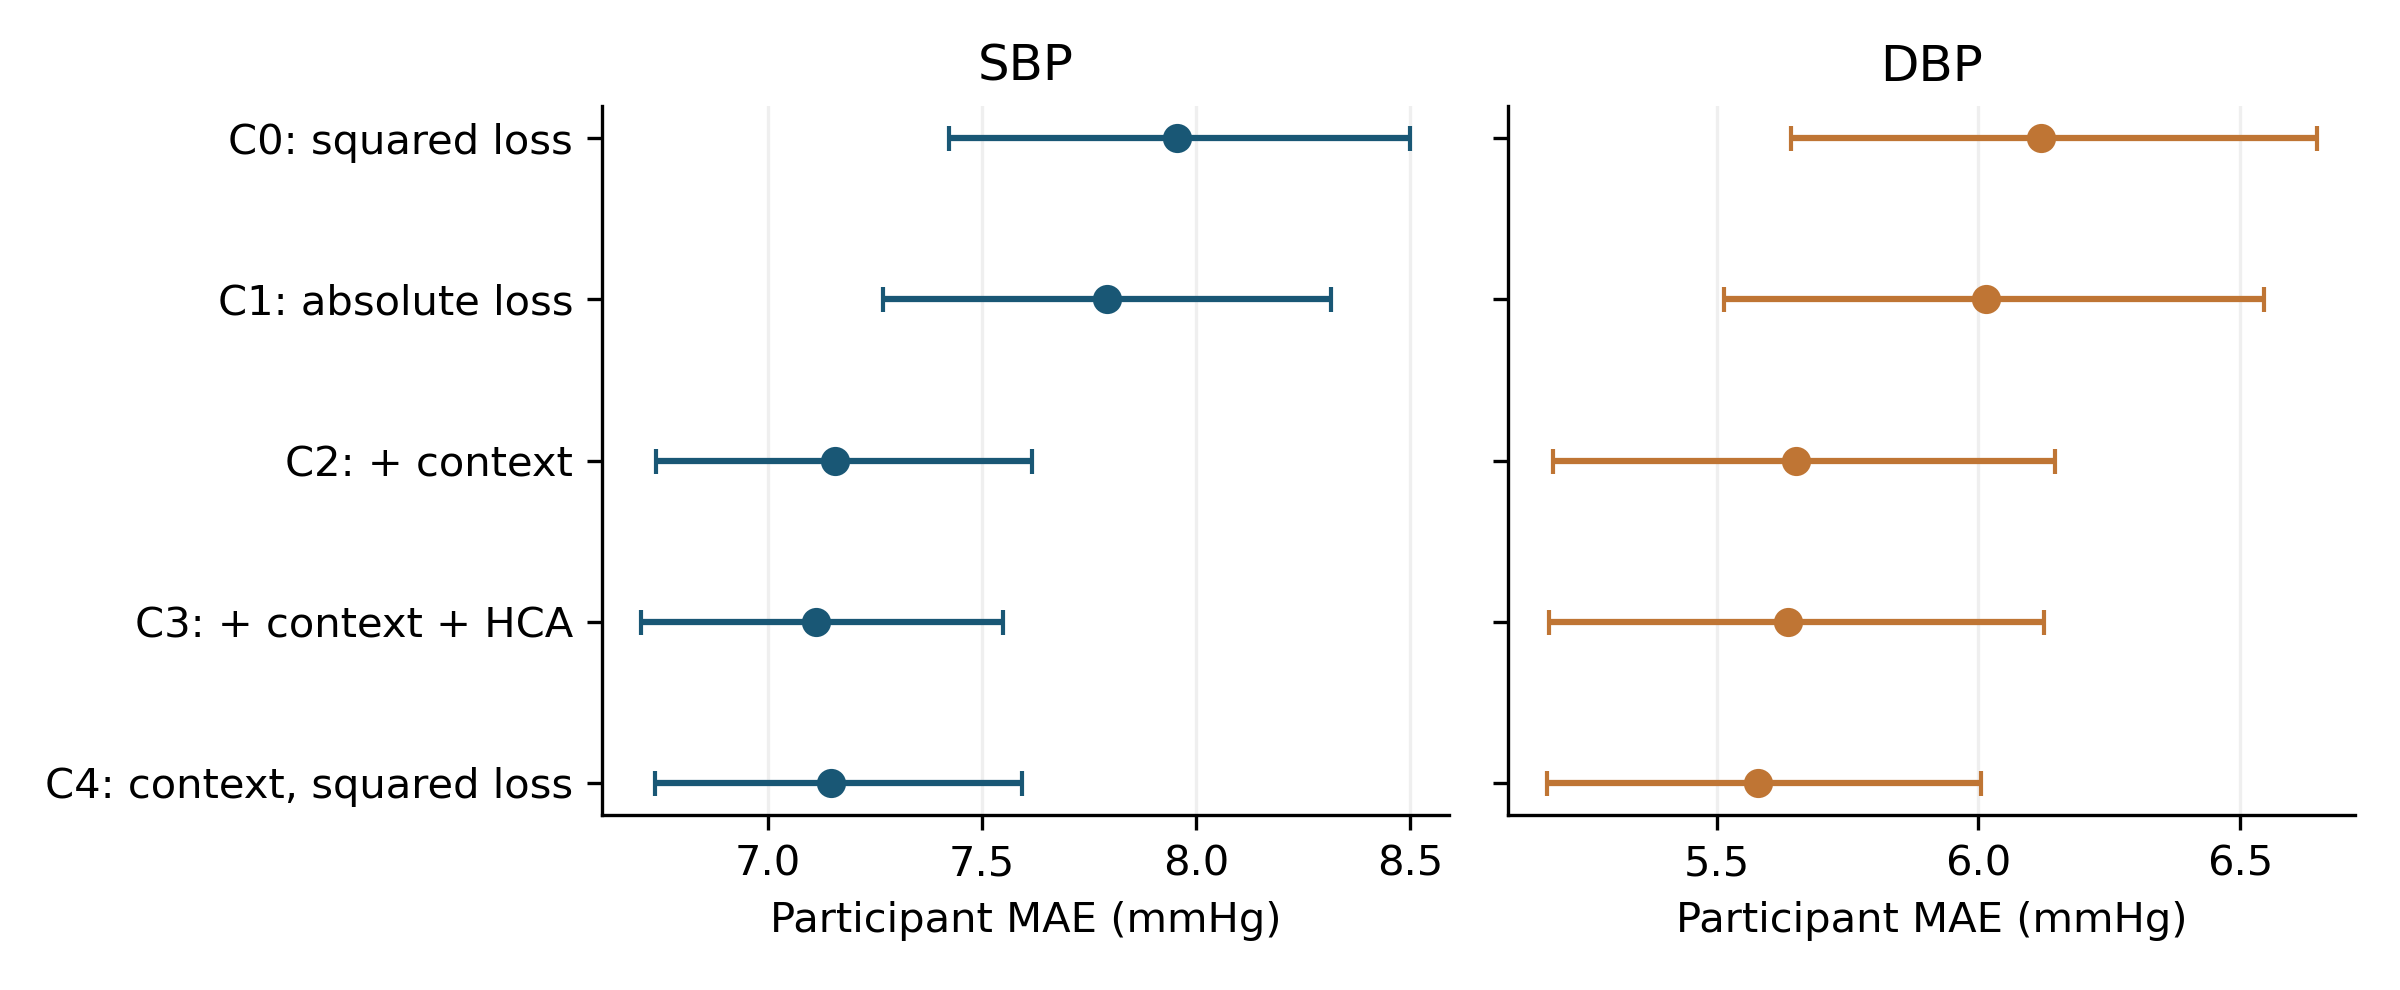
\includegraphics[width=\linewidth]{figures/fig_ladder.png}
\caption{Historical fixed-split session-anchored ladder with 95\% participant-bootstrap CIs. This figure documents model development; the main manuscript's primary validation table provides the primary repeated participant-validation result.}
\label{fig:ladder}
\end{figure}
\subsection{Calibration-Row Leakage Audit}
\label{sec:leakage-results}
Table~\ref{tab:leakage} reports all four checks from the main manuscript's calibration-row leakage audit. Check A shows calibration-flagged rows are smaller in mean $|\Delta|$ than unflagged rows ($6.774$ vs.\ $9.902$~mmHg SBP, development set) but not trivially near-zero, and the fraction of rows within 1~mmHg is nearly identical between flagged and unflagged rows ($9.8\%$ vs.\ $8.6\%$). The decisive Check D -- flag removed from features, flagged rows excluded from both fit and scoring -- yields a context gain of $+0.614$~mmHg SBP $[0.346, 0.889]$ and $+0.513$~mmHg DBP $[0.268, 0.743]$, both CI-supported and close to the unaudited historical figures. Leave-one-out attribution (Figure~\ref{fig:loo}) shows larger predictive contributions from recording duration and post-exercise activity, not the calibration flag (LOO damage for the flag: $0.0000$ SBP / $0.0027$ DBP).
\begin{table}[t]
\centering
\caption{Calibration-Row Leakage Audit (168 holdout participants)}
\label{tab:leakage}
\scriptsize
\resizebox{\columnwidth}{!}{%
\begin{tabular}{p{2.3cm}p{2.0cm}p{2.0cm}c}
\toprule
Check & SBP gain [CI] & DBP gain [CI] & Verdict \\
\midrule
B (flagged excl.) & 0.741 [0.440, 1.062] & 0.606 [0.372, 0.854] & Supp. \\
C (flag dropped) & 0.809 [0.501, 1.122] & 0.538 [0.309, 0.770] & Supp. \\
\textbf{D (strict)} & \textbf{0.614 [0.346, 0.889]} & \textbf{0.513 [0.268, 0.743]} & \textbf{Supp.} \\
\bottomrule
\end{tabular}
}
\end{table}
\begin{figure}[t]
\centering
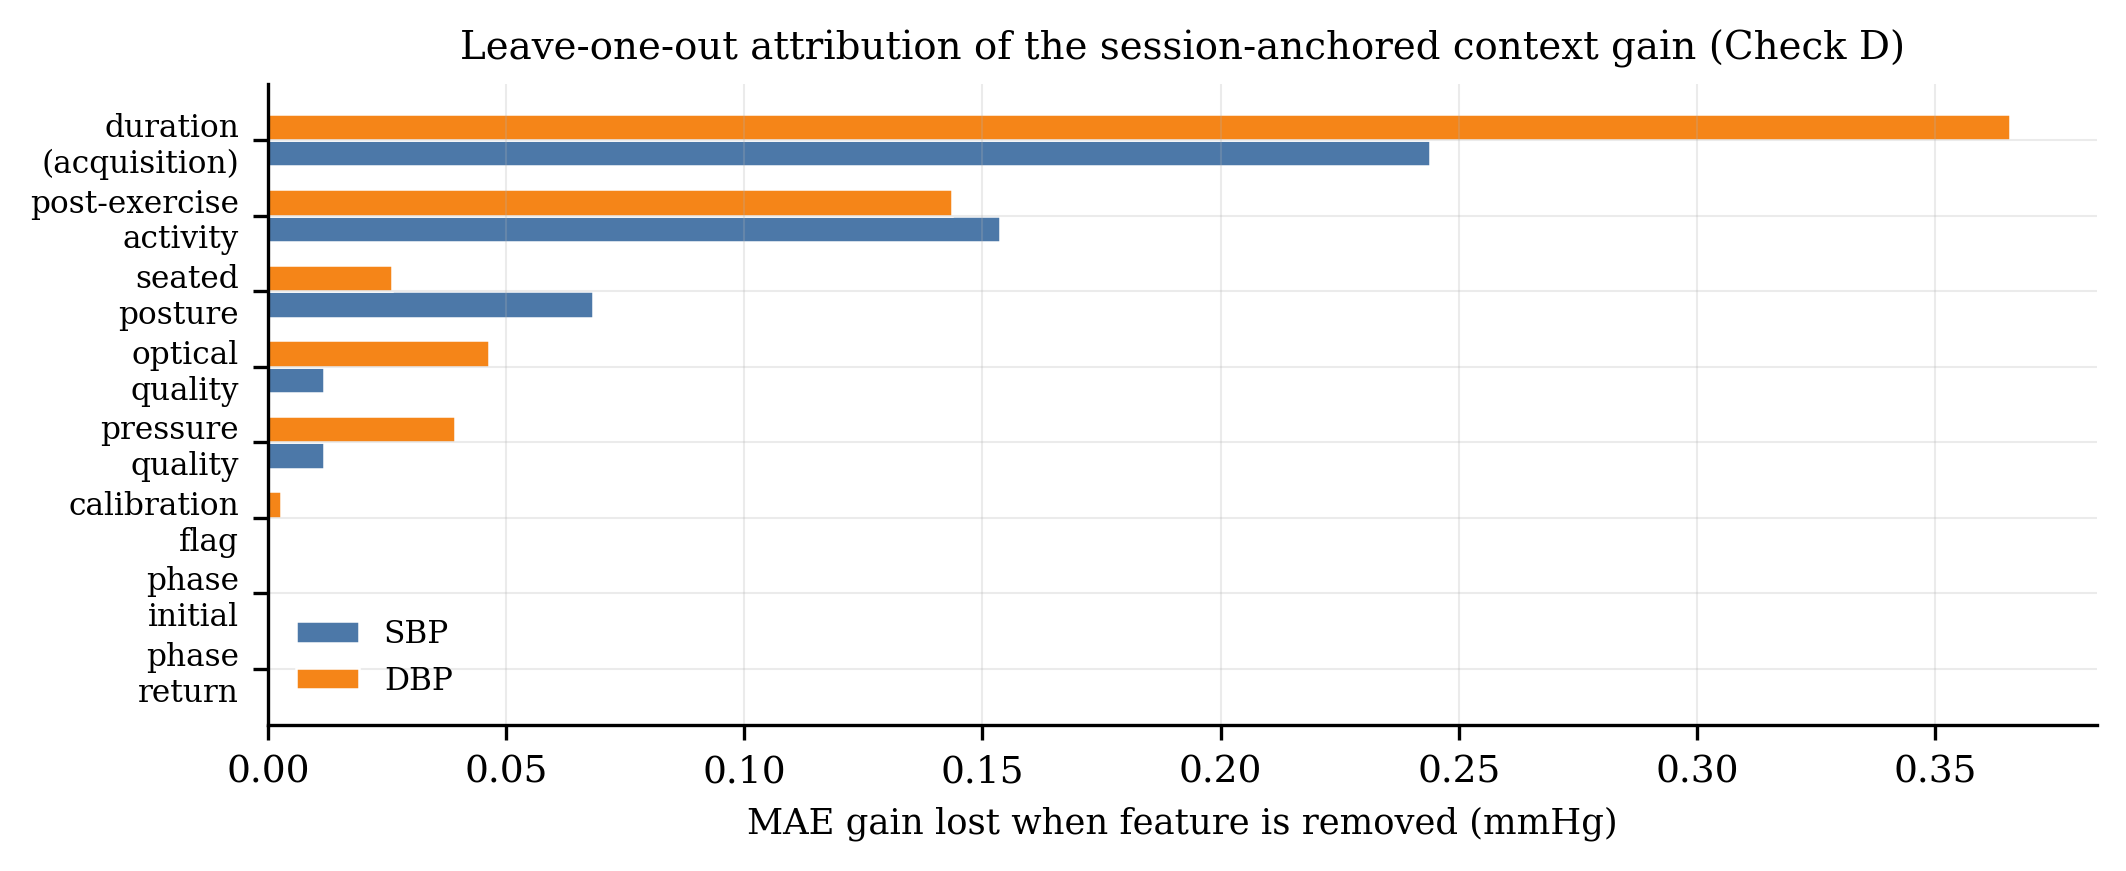
\includegraphics[width=\linewidth]{figures/fig_loo_context.png}
\caption{Leave-one-out attribution of the session-anchored context gain (Check D). The largest contributor is recording duration -- an acquisition property, not a purely physiological one -- followed by post-exercise activity.}
\label{fig:loo}
\end{figure}
One honest qualification: the single largest contributor to the context gain is recording \emph{duration} ($0.244$~mmHg SBP / $0.366$~mmHg DBP of leave-one-out damage), which is an acquisition property (likely proxying protocol step or signal stability) rather than a purely physiological state variable. ``Context = posture and activity'' is only partly right; post-exercise activity ($0.154$/$0.144$~mmHg) is the clearest genuinely physiological contributor, with posture third.

\subsection{Clinical Standards Context}
Table~\ref{tab:bhsaami} reports BHS grading and AAMI/ISO~81060-2 Criterion~1 for the C4 session-anchored model. The model improves cumulative within-5/10/15~mmHg percentages over both calibration retention and the legacy baseline for both SBP and DBP, and reaches BHS Grade~B for DBP (Grade~C for SBP); it passes AAMI Criterion~1 for DBP (mean error $0.645$, SD $7.992 \leq 8$~mmHg) but not for SBP (SD $9.654 > 8$~mmHg). \textbf{We report both gradings as indicative context, not a validation claim}: BHS and AAMI/ISO were written for cuff devices measuring absolute BP against an independent reference, and this model is calibrated per participant.
\begin{table}[t]
\centering
\caption{BHS Grading and AAMI/ISO 81060-2 Criterion 1 (Session-Anchored C4 Model, Measurement-Level)}
\label{tab:bhsaami}
\scriptsize
\resizebox{\columnwidth}{!}{%
\begin{tabular}{lccccc}
\toprule
Target/Arm & $\leq$5mm & $\leq$10mm & $\leq$15mm & Grade & AAMI-1 \\
\midrule
SBP calibration & 45.9\% & 72.3\% & 83.9\% & D & Fail \\
SBP baseline (C0) & 45.8\% & 73.8\% & 86.6\% & C & Fail \\
SBP model (C4) & 48.0\% & 75.1\% & 89.7\% & C & Fail \\
DBP calibration & 56.0\% & 82.9\% & 92.2\% & B & Fail \\
DBP baseline (C0) & 56.0\% & 83.1\% & 93.6\% & B & Fail \\
DBP model (C4) & 58.7\% & 85.6\% & 94.9\% & B & \textbf{Pass} \\
\bottomrule
\end{tabular}
}
\end{table}
\subsection{What Did Not Work}
\label{sec:whatdidnotwork}
Table~\ref{tab:whatdidnotwork} summarizes every intervention tested and rejected in this study, alongside one passed sanity check. We regard this table as carrying as much evidentiary weight as Table~\ref{tab:v23}: a result that survives repeated, adversarially-minded attempts to break it is more credible than one presented without them.


\subsection{Refitted Fixed-Estimator and Primary-Cohort Subgroups}
The historical prior-anchored estimator was refitted under the recorded environment, and Table~\ref{tab:fixedfst} reports its newly generated predictions. These estimates supersede the earlier rounded subgroup values; they do not assert bitwise recovery of the original run. The companion change record retains the old-value comparison. The same estimator is applied within each analysis before predictions are grouped by Fitzpatrick band. The primary wearable-state summary uses the independently regenerated repeated-CV predictions, not the historical fixed split.
\begin{table*}[t]
\centering
\caption{Regenerated Participant MAE by Fitzpatrick Band}
\label{tab:fixedfst}
\scriptsize
\resizebox{0.62\textwidth}{!}{%
\begin{tabular}{lllrr}
\toprule
Analysis & Target & Band ($n$) & MAE & 95\% CI \\
\midrule
Prior refit & SBP & I--II (133) & 5.837 & [5.513, 6.178] \\
Prior refit & SBP & III--IV (29) & 5.568 & [4.703, 6.549] \\
Prior refit & SBP & V--VI (6) & 5.341 & [3.847, 6.841] \\
Prior refit & DBP & I--II (133) & 4.439 & [4.118, 4.795] \\
Prior refit & DBP & III--IV (29) & 4.781 & [3.674, 6.370] \\
Prior refit & DBP & V--VI (6) & 4.020 & [2.931, 5.197] \\
\midrule
Primary CV & DBP & I--II (516) & 6.078 & [5.805, 6.362] \\
Primary CV & DBP & III--IV (112) & 6.435 & [5.862, 7.045] \\
Primary CV & DBP & V--VI (25) & 6.053 & [5.065, 7.122] \\
Primary CV & SBP & I--II (516) & 7.680 & [7.355, 8.022] \\
Primary CV & SBP & III--IV (112) & 7.786 & [7.050, 8.610] \\
Primary CV & SBP & V--VI (25) & 7.646 & [6.052, 9.471] \\
\bottomrule
\end{tabular}}
\end{table*}
These are exploratory marginal intervals. Differences in sample size, anchoring, and validation design prevent direct comparison between the two analysis blocks. In particular, the small V--VI samples do not establish parity or equivalence, irrespective of the ordering of the point estimates.

\end{document}
